\documentclass[a4paper,10pt]{article}
\usepackage[utf8]{inputenc}
\usepackage{polski}
\usepackage{graphicx}
\usepackage{listings}
\usepackage[usenames,dvipsnames]{color}
\addtolength{\hoffset}{-1cm}
\addtolength{\voffset}{-2cm}
\addtolength{\textwidth}{2cm}
\addtolength{\textheight}{3cm}
\usepackage{setspace}
\usepackage{indentfirst}
\usepackage{graphicx}
\lstset{
    language=Matlab,
    basicstyle=\scriptsize,
    aboveskip={1.5\baselineskip},
    columns=fixed,
    showstringspaces=false,
    extendedchars=true,
    breaklines=true,
    tabsize=4,
    prebreak = \raisebox{0ex}[0ex][0ex]{\ensuremath{\hookleftarrow}},
    frame=single,
    showtabs=false,
    showspaces=false,
    showstringspaces=false,
    identifierstyle=\ttfamily,
    keywordstyle=\color[rgb]{0,0,1},
    commentstyle=\color[rgb]{0.133,0.545,0.133},
    stringstyle=\color[rgb]{0.627,0.126,0.941},
    numbers=left,
    numberstyle=\tiny,
    stepnumber=1,
    numbersep=5pt,
    captionpos=b,
    escapeinside={\%*}{*)}
}

\def\figurename{Rys.}
\def\lstlistingname{Fun.}

\title{Informatyczne Systemy Sterowania \\ \large Ćwiczenie 3: Regulacja dwu- i trójpołożeniowa}

\author{Krzysztof Przybylski 239266}

\begin{document}
\maketitle

\section{Wstęp}\label{sec:wstęp}
\subsection{Cel ćwiczenia}
Celem tego ćwiczenia jest symulacja działania systemu regulacji z przekaźnikami dwu- i trójpołożeniowymi. Ćwiczenie ma umożliwić zapoznanie się z nieliniowymi algorytmami sterowania (przełącznikami dwu- i trójpołożeniowymi) oraz zapoznanie się ze środowiskiem Simulink oraz Matlab w zakresie nieliniowych algorytmów sterowania.
%Czy to jest dobrze?

\subsection{Plan badań} 
\begin{enumerate}
	\item Symulacja systemu regulacji. Dobór parametrów regulatora. \newline
	%czy to jest poprawne gramatycznie? :P
	 \small {W trakcie realizacji zadania należy zasymulować działanie systemu regulacji pracującego z regulatorem oraz należy zbadać wpływ wartości parametrów przekaźników na przebieg błędu regulacji}
	\begin{enumerate}
		\item Regulator dwupołożeniowy bez histerezy.
		\item Regulator dwupołożeniowy z histerezą.
		\item Regulator trójpołożeniowy bez histerezy.
		\item Regulator trójpołożeniowy z histerezą.
 	\end{enumerate}
	\item Zastosowanie członów korekcyjnych.
	\begin{enumerate}
		\item Modyfikacja systemów z zadania 1 o korekcję w postaci członu liniowego o transmitancji: 
			\begin{equation} \label{eqn:czlonKorekcyjny}
				K_{k}(s) = {{k_{k}} \over {T_{k}s+1}}
			\end{equation}
		\item Doświadczalny dobor parametrów członu korekcyjnego.
	\end{enumerate}
\end{enumerate}

\newpage
\section{Realizacja planu i wyniki}
%--------------------------------------------------------------------------------------------------------------------------------
%ZADANIE 1
%--------------------------------------------------------------------------------------------------------------------------------
\subsection{Symulacja systemu regulacji. Dobór parametrów regulatora.}\label{sec:zad1}

System regulacji będziemy symulować przy użyciu programu Simulink będącego częścią pakietu M\small ATLAB.\normalsize

\subsubsection{Regulator dwupołożeniowy bez histerezy}\label{sec:r2bh}
%--------------------------------------------------------------------------------------------------------------------------------

Schemat systemu do symulacji regulatora dwupołożeniowego przedstawiony został na poniższym rysunku.

\begin{figure}[!h]
    \centering
	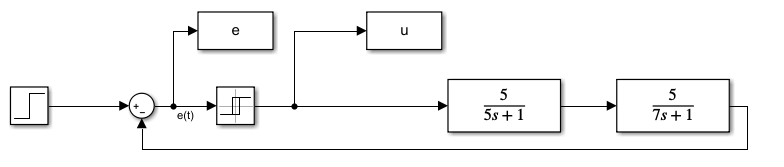
\includegraphics[width=120mm]{dwu_schemat.png}
	\caption{Schemat symulacji regulatora dwupołożeniowego.}
    \label{fig:Rysunek}
\end{figure}

Aby zasymulować regulator dwupołożeniowy bez histerezy trzeba ustawić parametry 'On' i 'Off' obiektu 'Relay' na wartość 0. \\
Za przeprowadzenie testu odpowiedzialna jest poniższa funkcja.

\begin{lstlisting}[caption=Funkcja testująca regulator dwupołożeniowy bez histerezy.]
function testDwupolozeniowyBezHisterezy()
load_system('dwupolozeniowy.slx');
hold on;

set_param('dwupolozeniowy/Relay', 'OnSwitchValue', num2str(0));
set_param('dwupolozeniowy/Relay', 'OffSwitchValue', num2str(0));

sim('dwupolozeniowy.slx');
figure(1);
plot(u.time, u.signals.values, '-r');
figure(2);
plot(e.time, e.signals.values, '-k');
end
\end{lstlisting}

Po wywołaniu tej funkcji otrzymałem poniższe wykresy.

\begin{figure}[!h]
    \centering
	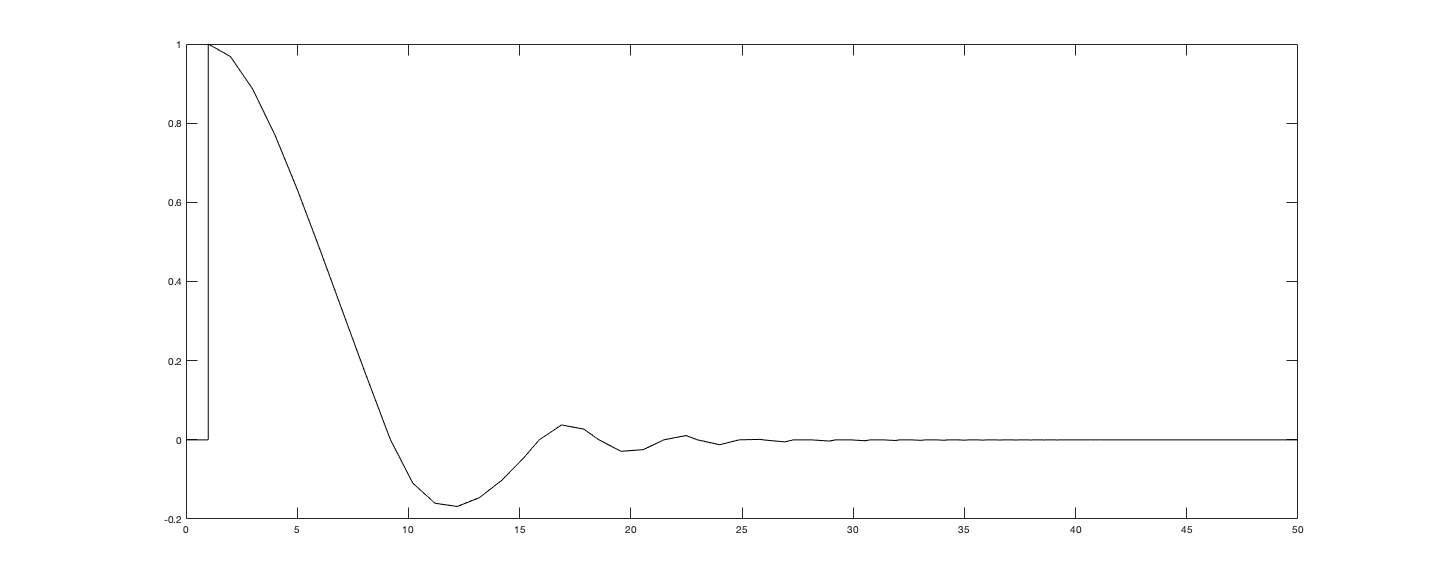
\includegraphics[width=120mm]{dwu_bez_his_e.png}
	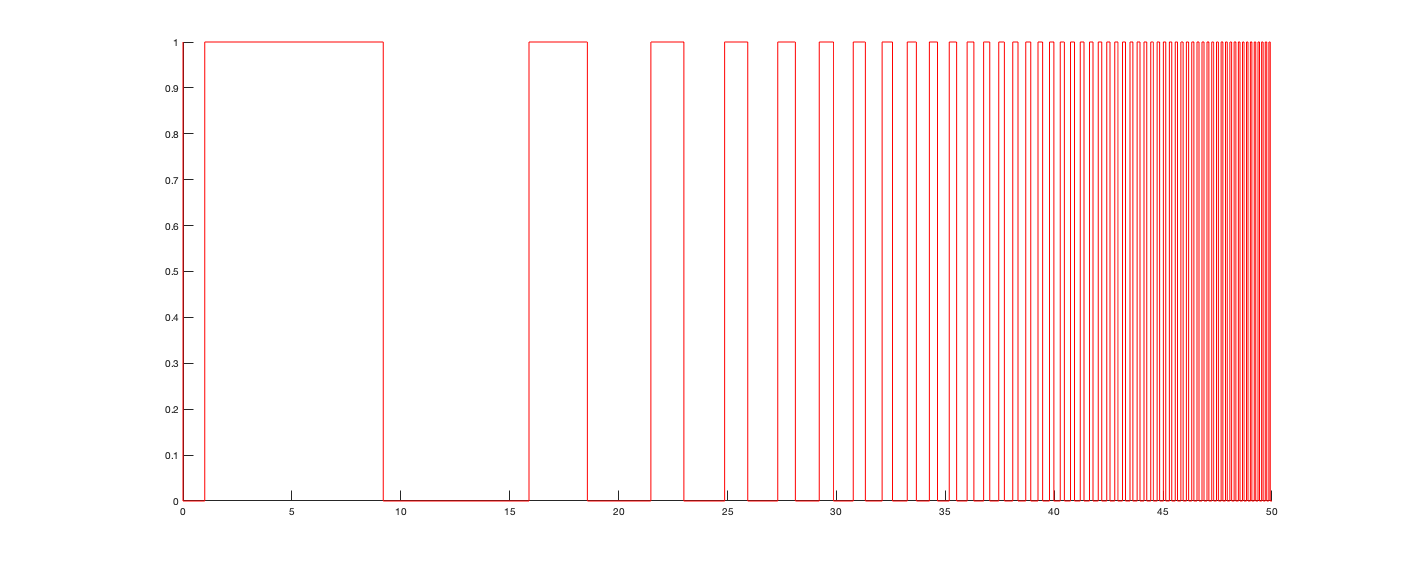
\includegraphics[width=120mm]{dwu_bez_his_u.png}
	\caption{Wykresy $\varepsilon(t)$, oraz $u(t)$ dla regulatora dwupołożeniowego bez histerezy.}
    \label{fig:Rysunek}
\end{figure}

\newpage Widać z nich, że wykres błędu oscyluje z czasem coraz bliżej zera, więc wartość na wyjściu jest blisko pożądanej, lecz z czasem rośnie również częstotliwość przełączania regulatora, przez co znacznie rośnie jego zużycie i maleje żywotność.

\subsubsection{Regulator dwupołożeniowy z histerezą}\label{sec:r2h}
%--------------------------------------------------------------------------------------------------------------------------------

Histereza dwupoziomowa sprawia, że przełączanie stanu z wysokiego na niski nie zachodzi przy tej samej wartości co przełączanie stanu z niskiego na wysoki. Jej działanie przedstawione zostało na poniższym obrazku.

\begin{figure}[!h]
    \centering
	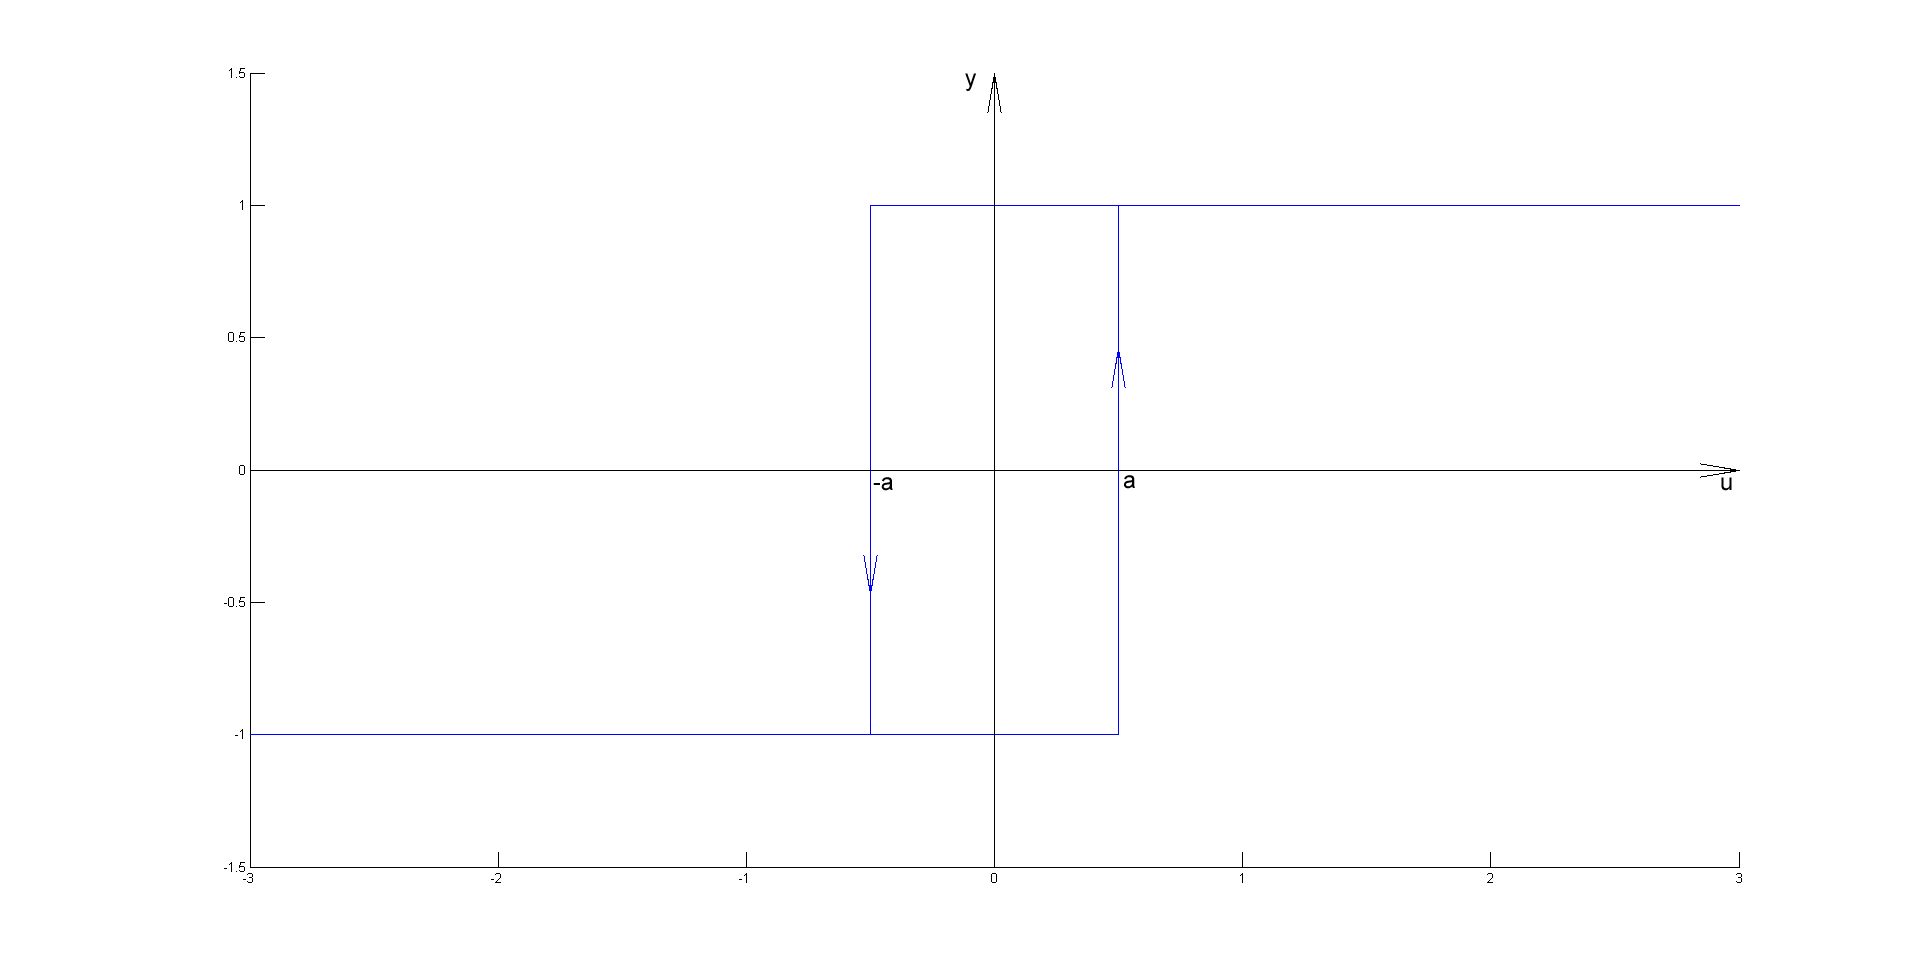
\includegraphics[width=120mm]{CW3-histereza-dwupoziomowa.png}
	\caption{Jak działa histereza dwupoziomowa.}
    \label{fig:Rysunek}
\end{figure}

Symulacje regulatora dwupoziomowego z histerezą przeprowadzę na tym samym modelu, który posłużył mi w zadaniu \ref{sec:r2bh}, jednak w obiekcie 'Relay' parametry 'On' i 'Off' będą różne, dzięki czemu ustawimy żądaną histerezę.\newpage
Za przeprowadzenie testu odpowiedzialna jest poniższa funkcja.

\begin{lstlisting}[caption=Funkcja testująca regulator dwupołożeniowy z histerezą.]
function testDwupolozeniowyZHistereza(step, stop, drawU)
load_system('dwupolozeniowy.slx');
hold on;
i = step;

while (i <= stop)
set_param('dwupolozeniowy/Relay', 'OnSwitchValue', num2str(i));
set_param('dwupolozeniowy/Relay', 'OffSwitchValue', num2str(-i));

sim('dwupolozeniowy.slx');
figure(1);

plot(e.time, e.signals.values, 'DisplayName', strcat('a=', num2str(i)));

if drawU
figure(2);
plot(u.time, u.signals.values);
end

i=i+step;
hold all;
end
end
\end{lstlisting}

Po wywołaniu powyższej funkcji dla wartości (0.5, 0.6, true) otrzymałem poniższe wykresy.

\begin{figure}[!h]
    \centering
	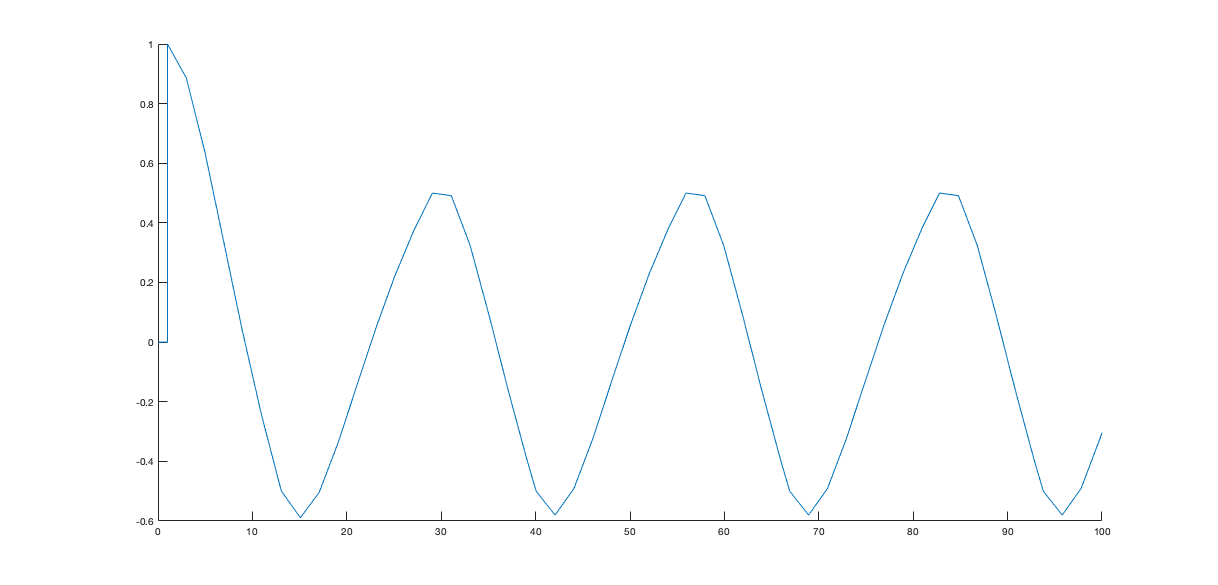
\includegraphics[width=120mm]{dwu_z_his_e.png}
	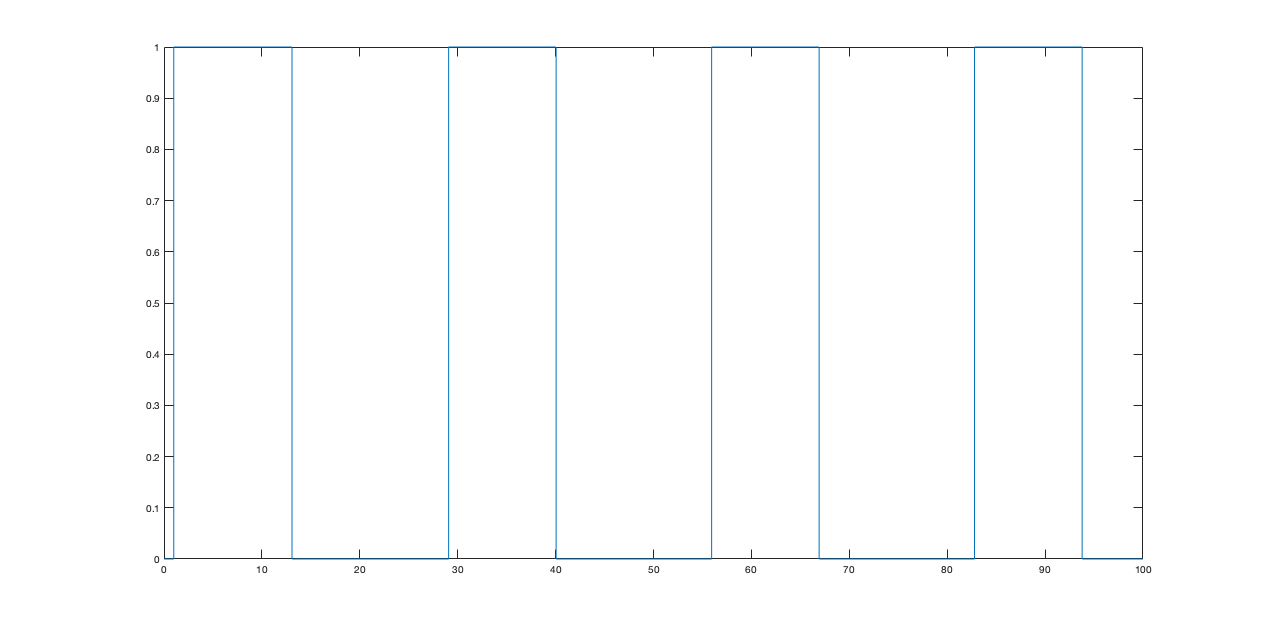
\includegraphics[width=120mm]{dwu_z_his_u.png}
	\caption{Wykresy $\varepsilon(t)$, oraz $u(t)$ dla regulatora dwupołożeniowego z histerezą.}
    \label{fig:Rysunek}
\end{figure}

Widać na nich, że amplituda oscylacji błędu wokół zera z czasem stabilizuje się, a liczba przełączeń znacznie maleje w stosunku do regulatora dwupołożeniowego bez histerezy, a więc i wydłuża się jego żywotnosć. \\
Aby zbadać wpływ zakresu histerezy na wykres $\varepsilon(t)$ wywołałem funkcję dla wartości (0.2, 0.8, false), w wyniku czego otrzymałem poniższe wykresy.

\begin{figure}[!h]
    \centering
	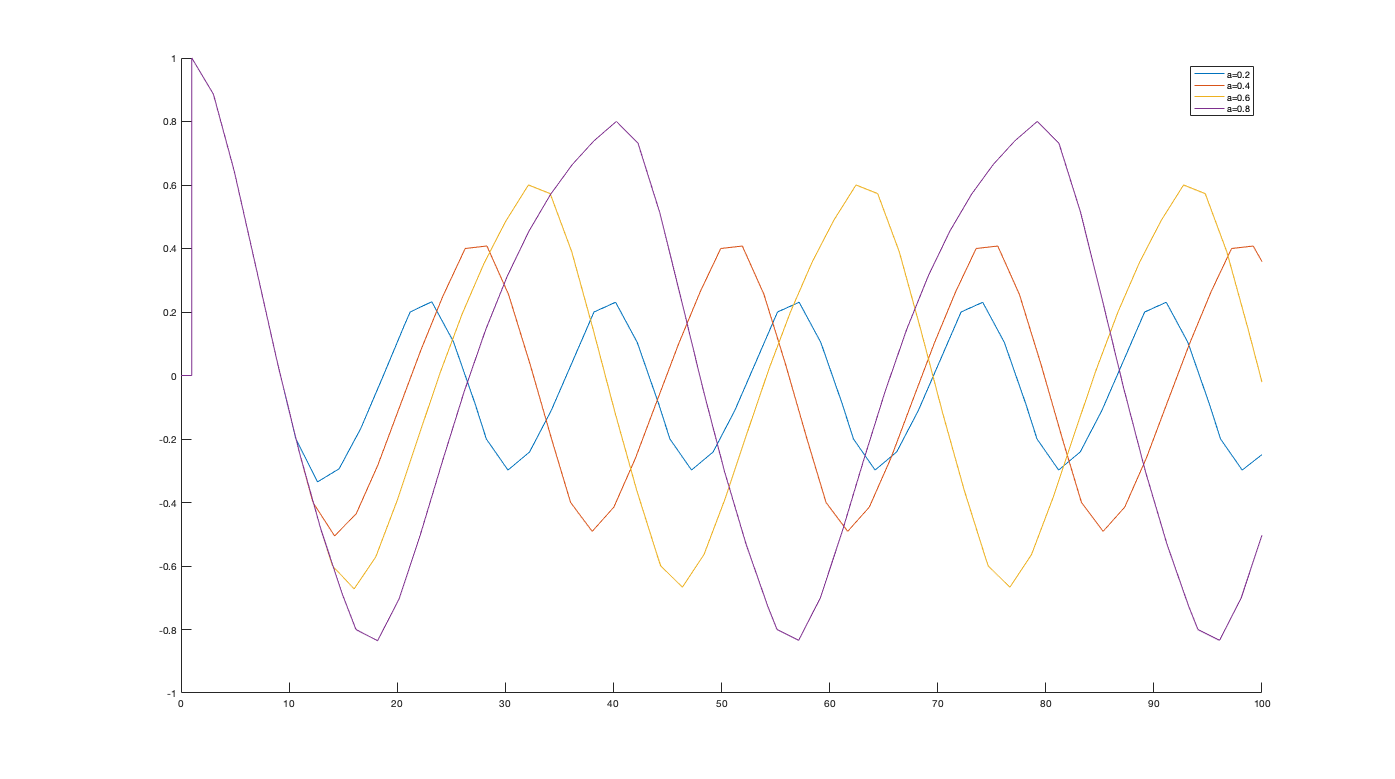
\includegraphics[width=120mm]{dwu_z_his_e_2.png}
	\caption{Wykres $\varepsilon(t)$ dla regulatora dwupołożeniowego z histerezą przy rosnącym $a$.}
    \label{fig:Rysunek}
\end{figure}

\newpage Widać na nich, że w miarę zwiększania zakresu histerezy rośnie amplituda oscylacji wykresu błędu wokół zera, oraz maleje częstotliwość przełączeń regulatora.

\subsubsection{Regulator trójpołożeniowy bez histerezy}\label{sec:r3bh}
%--------------------------------------------------------------------------------------------------------------------------------

\normalsize Schemat systemu do symulacji regulatora trójpołożeniowego przedstawiony został na poniższym rysunku.

\begin{figure}[!h]
    \centering
	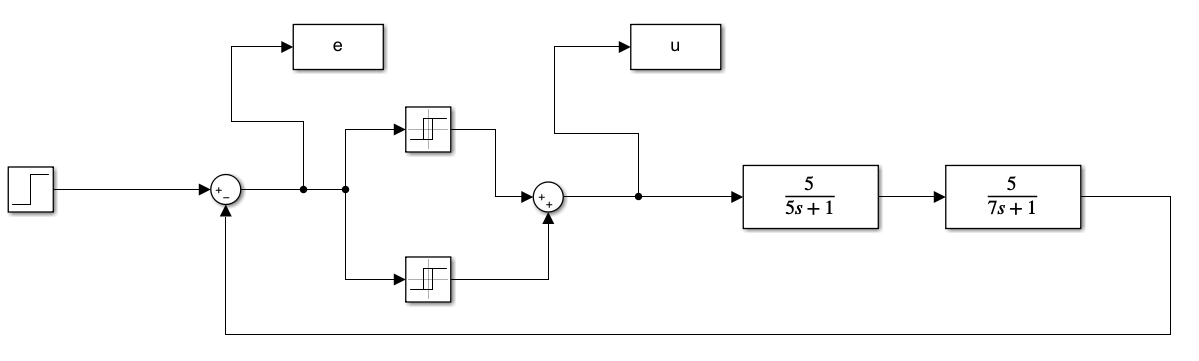
\includegraphics[width=120mm]{troj_schemat.png}
	\caption{Schemat symulacji regulatora trójpołożeniowego.}
    \label{fig:Rysunek}
\end{figure}

Aby zasymulować regulator trójpołożeniowy bez histerezy nalezy parametry 'On' i 'Off' obiektów 'Relay1' i 'Relay2' na wartość 0.
\newpage Za przeprowadzenie testu odpowiedzialna jest poniższa funkcja.

\begin{lstlisting}[caption=Funkcja testująca regulator trójpołożeniowy bez histerezy.]
function testTrojpolozeniowyBezHisterezy()
load_system('trojpolozeniowy.slx');
hold on;


set_param('trojpolozeniowy/Relay1', 'OnSwitchValue', num2str(0));
set_param('trojpolozeniowy/Relay1', 'OffSwitchValue', num2str(0));
set_param('trojpolozeniowy/Relay2', 'OnSwitchValue', num2str(0));
set_param('trojpolozeniowy/Relay2', 'OffSwitchValue', num2str(0));


sim('trojpolozeniowy.slx');
figure(1);
plot(u.time, u.signals.values);
plot(e.time, e.signals.values);
%plot(fun.time, fun.signals.values);
end
\end{lstlisting}

Po wywołaniu tej funkcji otrzymałem poniższy wykres.

\begin{figure}[!h]
    \centering
	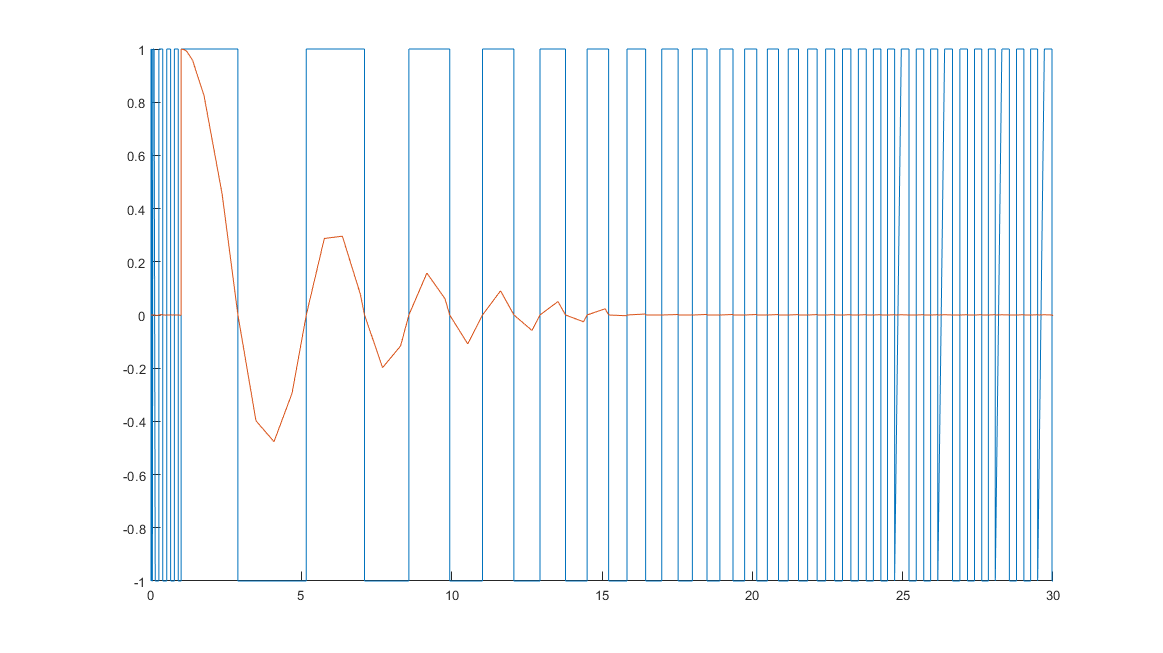
\includegraphics[width=120mm]{troj_bez_his.png}
	\caption{Wykresy $\varepsilon(t)$, oraz $u(t)$ dla regulatora trójpołożeniowego bez histerezy.}
    \label{fig:Rysunek}
\end{figure}

\newpage Widać z nich, że wykres błędu oscyluje z czasem coraz bliżej zera, więc wartość na wyjściu jest blisko pożądanej, lecz z czasem rośnie również częstotliwość przełączania regulatora, przez co znacznie rośnie jego zużycie i maleje żywotność. \\
Widać również, że regulator trójpołożeniowy nie wszedł w stan zerowy ani razu. Dzieje się tak, ponieważ przełączenia regulatora są zbyt szybkie.

\subsubsection{Regulator trójpołożeniowy z histerezą}\label{sec:r3h}
%--------------------------------------------------------------------------------------------------------------------------------

Histereza trójpoziomowa to nic innego niż połączenie dwóch histerez dwupoziomowych. Jej działanie przedstawione zostało na poniższym obrazku.

\begin{figure}[!h]
    \centering
	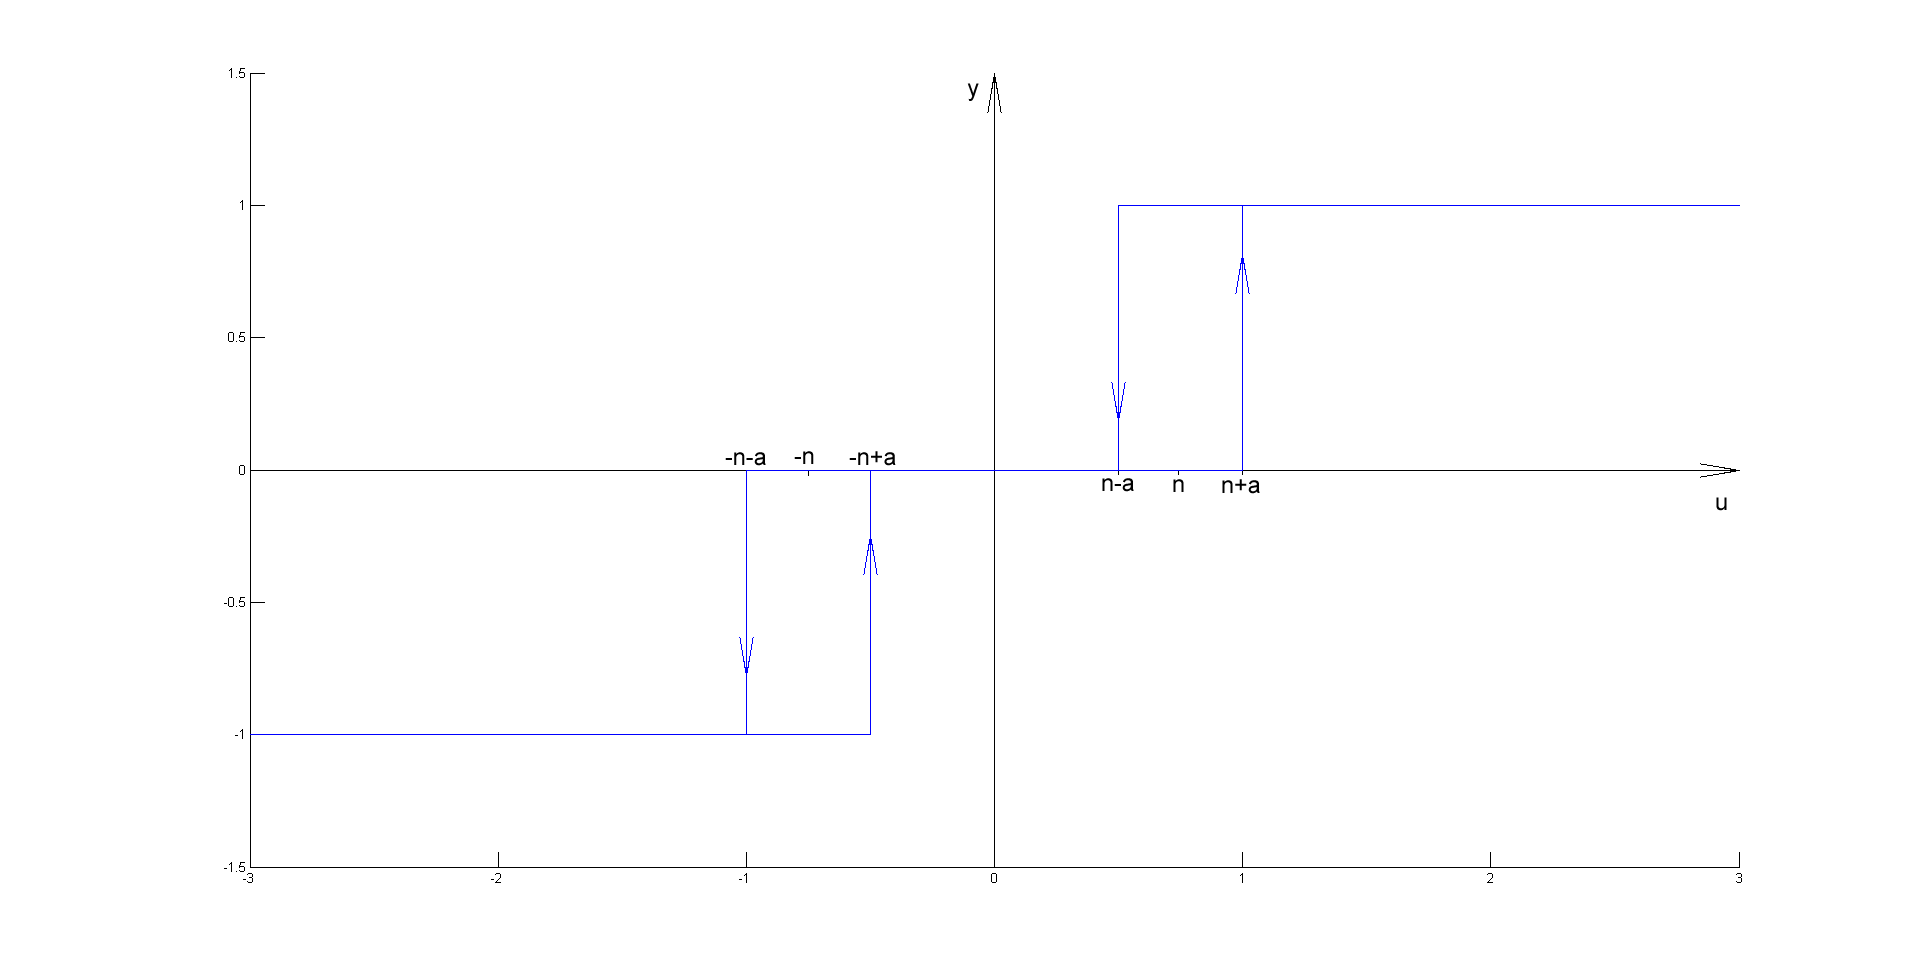
\includegraphics[width=120mm]{CW3-histereza-trojpoziomowa.png}
	\caption{Jak działa histereza trójpoziomowa.}
    \label{fig:Rysunek}
\end{figure}

Symulacje regulatora trójpołożeniowego z histerezą przeprowadzę na tym samym modelu, który posłużył mi w zadaniu \ref{sec:r3bh}, jednak w obiektach 'Relay1' i 'Relay2' parametry 'On' i 'Off' będą różne, dzięki czemu uzyskam żądaną histerezę.
Za przeprowadzenie testu odpowiedzialna jest poniższa funkcja.

\begin{lstlisting}[caption=Funkcja testująca regulator trójpołożeniowy z histerezą.]
function testTrojpolozeniowyZHistereza(start, step, stop)
load_system('trojpolozeniowy.slx');
hold on;
i = 1;

s1 = start;
s2 = start;
while(s1 <= stop)

s1 = s1 + step;
s2 = s2 - step;

set_param('trojpolozeniowy/Relay1', 'OnSwitchValue', num2str(s1*i));
set_param('trojpolozeniowy/Relay1', 'OffSwitchValue', num2str(s2*i));
set_param('trojpolozeniowy/Relay2', 'OnSwitchValue', num2str(-(s2*i)));
set_param('trojpolozeniowy/Relay2', 'OffSwitchValue', num2str(-(s1*i)));


sim('trojpolozeniowy.slx');
figure(1);
%plot(relay.time, relay.signals.values);
plot(e.time, e.signals.values, 'DisplayName', num2str(s1));
%plot(fun.time, fun.signals.values);
i = i +1;
end
hold all;
end
\end{lstlisting}

Po wywołaniu powyższej funkcji dla wartości (0.2, 0.1, 0.8) otrzymałem poniższy wykres.

\begin{figure}[!h]
    \centering
	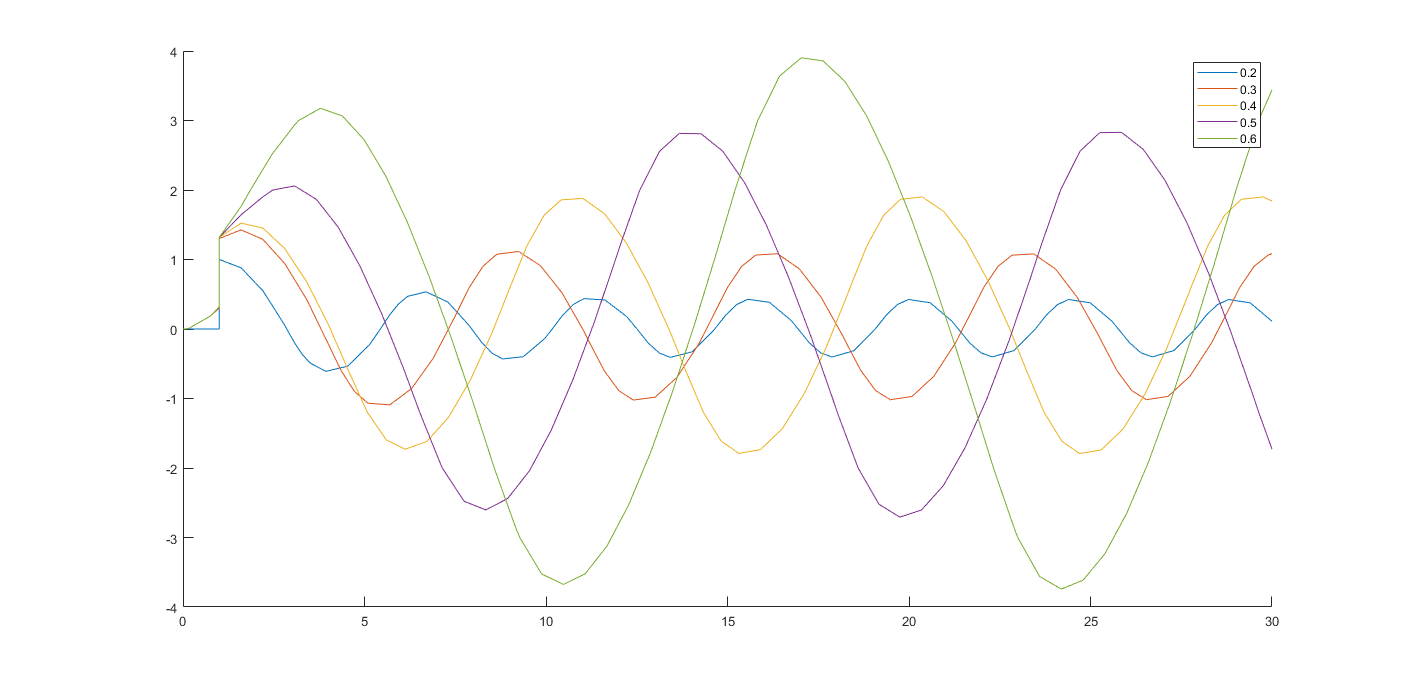
\includegraphics[width=120mm]{troj_z_his.png}
	\caption{Wykresy $\varepsilon(t)$, oraz $u(t)$ dla regulatora trójpołożeniowego z histerezą.}
    \label{fig:Rysunek}
\end{figure}

\newpage Widać na nim, że w miarę zwiększania zakresu histerezy rośnie amplituda oscylacji wokół zera wykresu błędu.

%---------------------------------------------------------------------------------------------------------------------
%ZADANIE 2
%---------------------------------------------------------------------------------------------------------------------

\subsection{Zastosowanie członów korekcyjnych.}\label{sec:zad2}
Podstawową zaletą regulacji dwupołożeniowej jest prostota realizacji. Niestety, cecha ta jest
okupiona pogorszeniem jakości parametrów regulacji w porównaniu regulacją ciągłą.
Jedną z możliwości poprawienia jakości regulacji jest zastosowanie układu z korekcją.
\newline
Człon korekcyjny posiada następującą transmitancję:

\begin{equation} \label{eqn:trans_czl_kor}
	G_w={{k} \over {T_k s+1}}
\end{equation}

\subsubsection{Modyfikacja systemów z zadania 1}\label{sec:zad2_1}
\begin{figure}[!h]
    \centering
	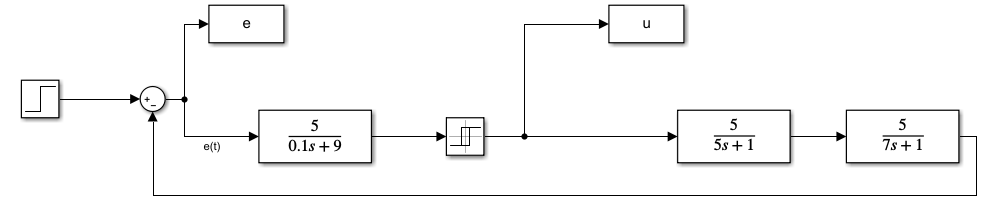
\includegraphics[width=120mm]{dwu_kor_schemat.png}
	\caption{Schemat regulatora dwupolożeniowego z korekcją.}
    \label{fig:Rysunek}
\end{figure}

\begin{figure}[!h]
    \centering
	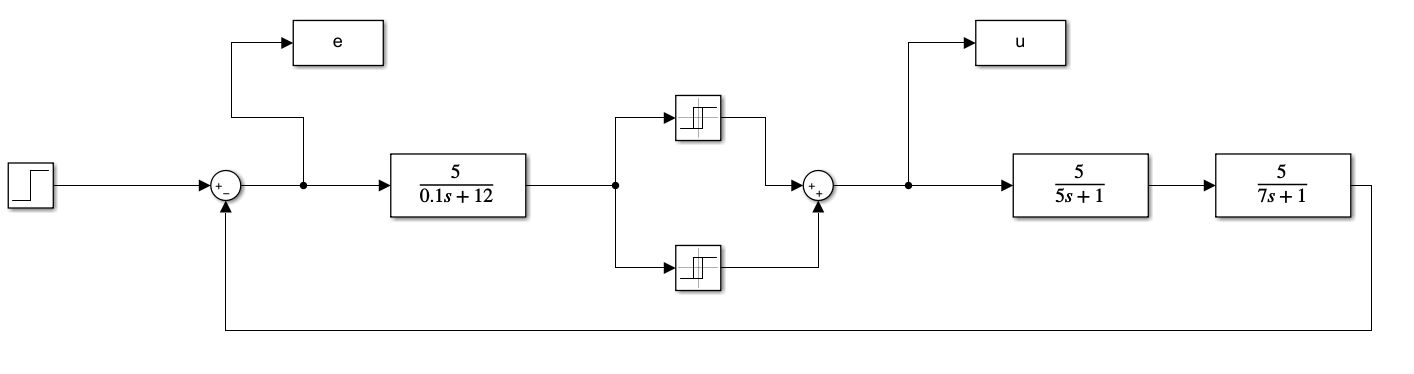
\includegraphics[width=120mm]{troj_kor_schemat.png}
	\caption{Schemat regulatora trojpolożeniowego z korekcją.}
    \label{fig:Rysunek}
\end{figure}
Człon korekcyjny powoduje modyfikację sygnału błędu dzięki czemu przełączanie następuje szybciej.
\newpage

\subsubsection{Doświadczalny dobor parametrów członu korekcyjnego.}\label{sec:zad2_2}
\begin{enumerate}
		\item Regulator dwupołożeniowy.
		
		Do sprawdzania regulatorów wykorzystałem następujące funkcje testujące.
		
\begin{lstlisting}[caption=Funkcja testująca regulator dwupoziomowy z korekcją zmiana T.]
function testDwupolozeniowyKor(start, step, stop)
load_system('dwupolozeniowy_kor.slx');
hold on;
s=start;


while(s <= stop)
set_param('dwupolozeniowy_kor/Transfer Fcn3', 'Denominator', strcat('[',num2str(s), ' 1]'));
%set_param('dwupolozeniowy_kor/Transfer Fcn3', 'Denominator', strcat("[0.1 ", num2str(s), ']'));
%set_param('dwupolozeniowy_kor/Transfer Fcn3', 'Denominator', strcat("[0.1 0.3]"));
sim('dwupolozeniowy_kor.slx');

figure(1);
plot(e.time, e.signals.values, 'DisplayName', strcat('k=',num2str(s)));
s= s+step;

end


hold all;


end
\end{lstlisting}

Analogicznie do testowania k

\begin{lstlisting}[caption=set param dla k.]
set_param('dwupolozeniowy_kor/Transfer Fcn3', 'Denominator', strcat("[0.1 ", num2str(s), ']'));
\end{lstlisting}
\newpage

Na początek testowany był układ z histerezą. Zadanie polegało on doświadczalnym dobraniu parametrów układu korekcyjnego.
Parametrami nas interesującymi są Tk, k.

\begin{figure}[!h]
    \centering
	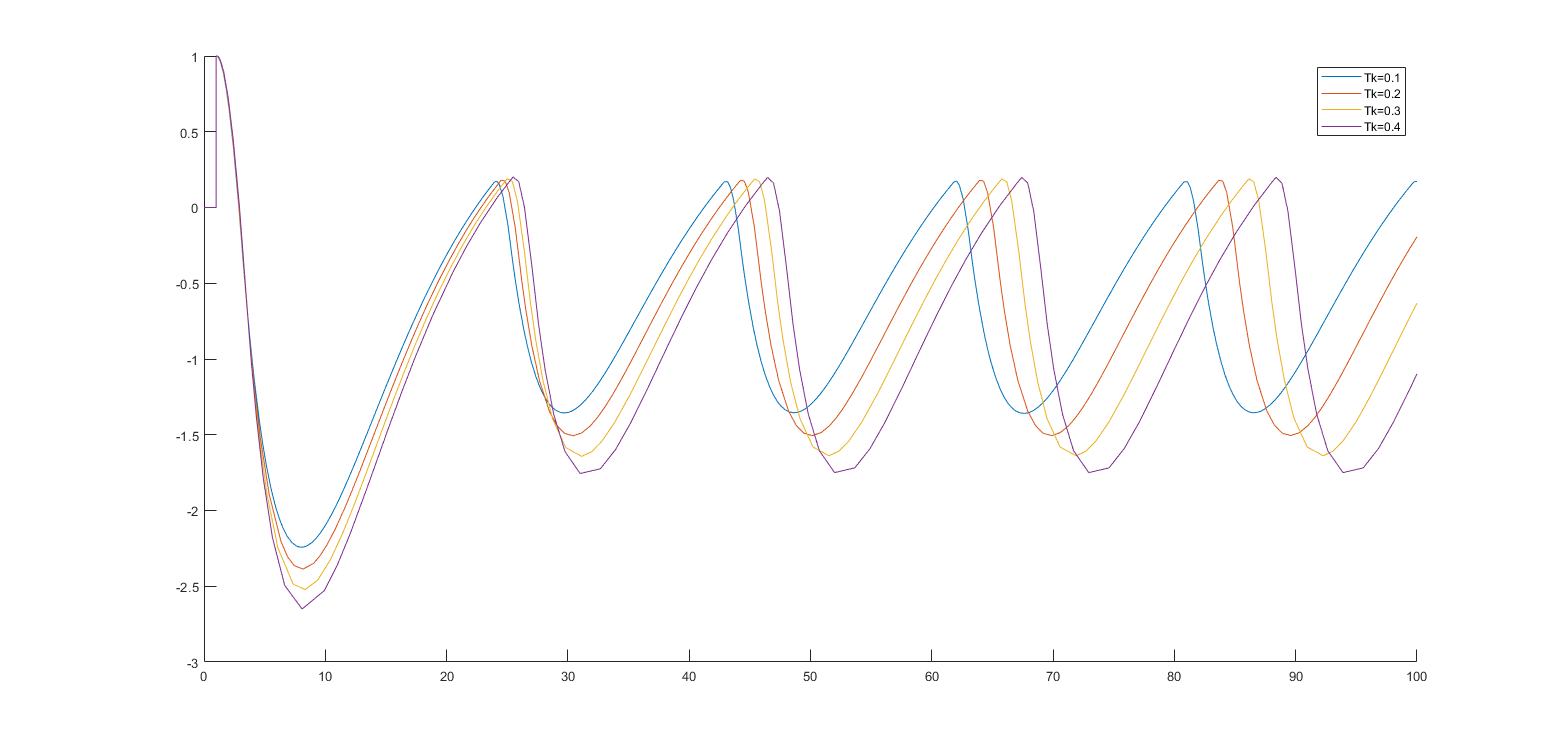
\includegraphics[width=120mm]{dwu_kor_tk.png}
	\caption{Zmiana Tk przy stałym k=1}
    \label{fig:Rysunek}
\end{figure}

Z wyresu można zauważyć, że dla wartości k=1, wartość optymalna Tk=0.1 ze względu na najmniejsze wachania wartości.

\begin{figure}[!h]
    \centering
	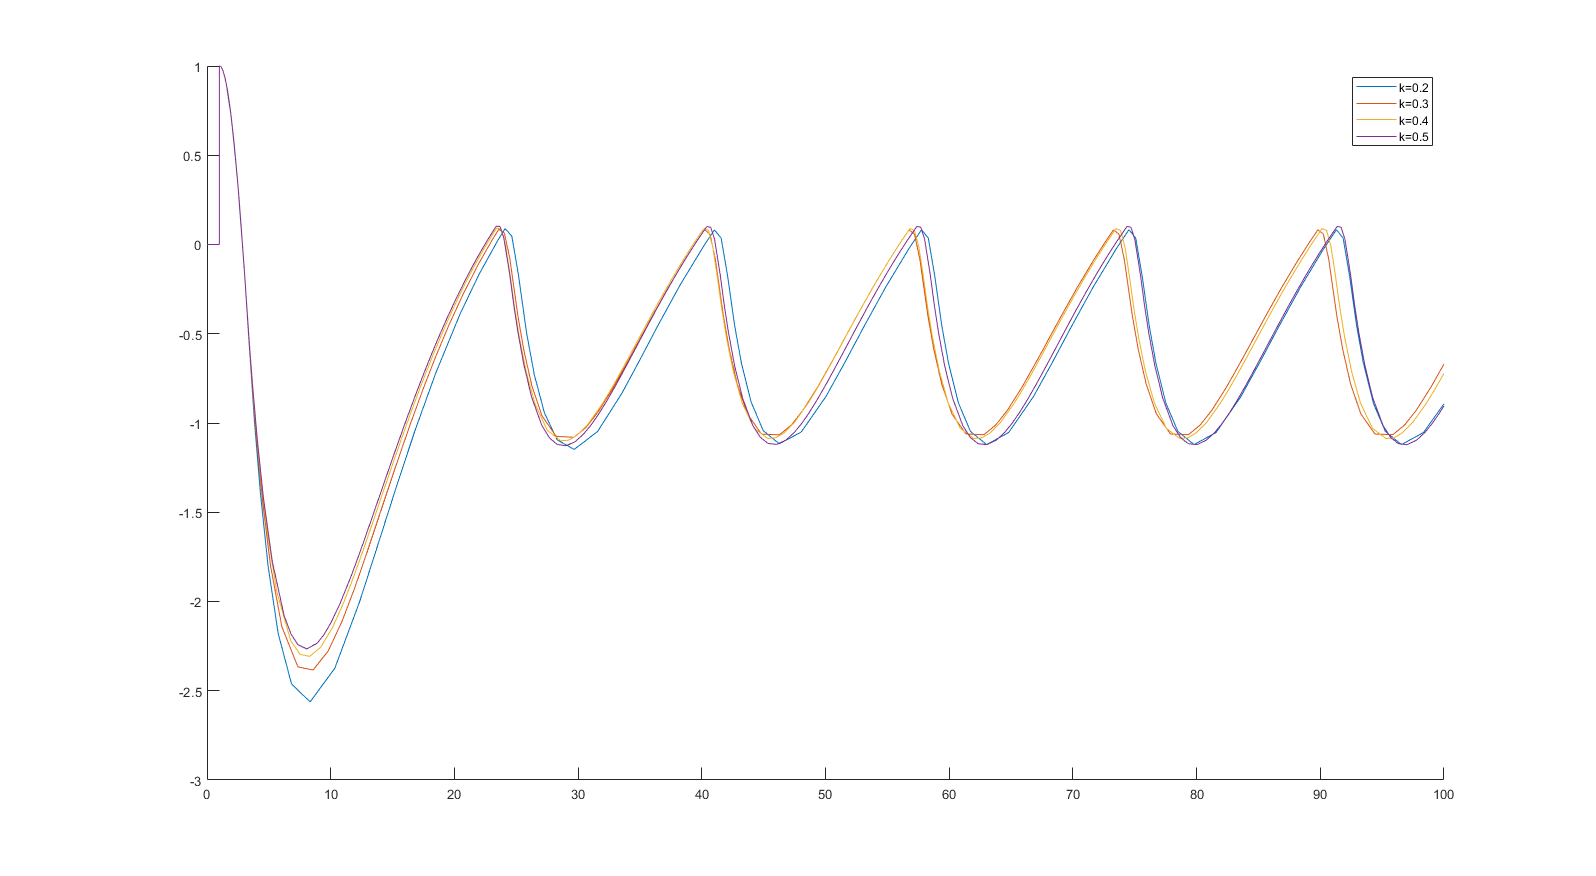
\includegraphics[width=120mm]{dwu_kor_k.png}
	\caption{Zmiana k przy stałym Tk=0.1}
    \label{fig:Rysunek}
\end{figure}
Gdy Tk=0.1 najbardziej optymalne k=0.3 ze względu, że oscyluje najmniej.
\newpage

Dla układu bez histerezy otrzymałem zbliżone wyniki:
\begin{figure}[!h]
    \centering
	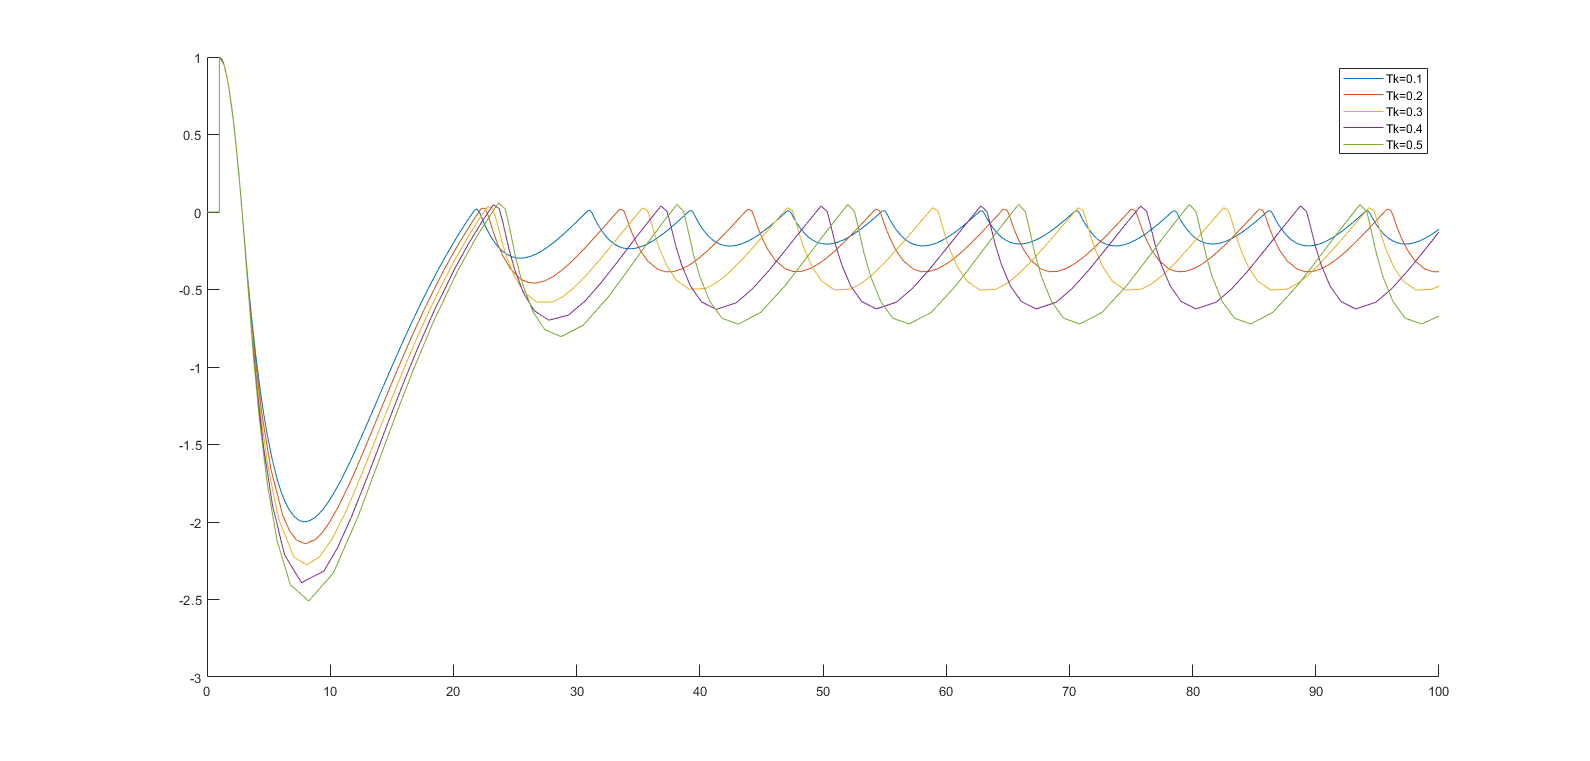
\includegraphics[width=120mm]{dwu_kor_tk_bez.png}
	\caption{Zmiana Tk przy stałym k=1}
    \label{fig:Rysunek}
\end{figure}

\begin{figure}[!h]
    \centering
	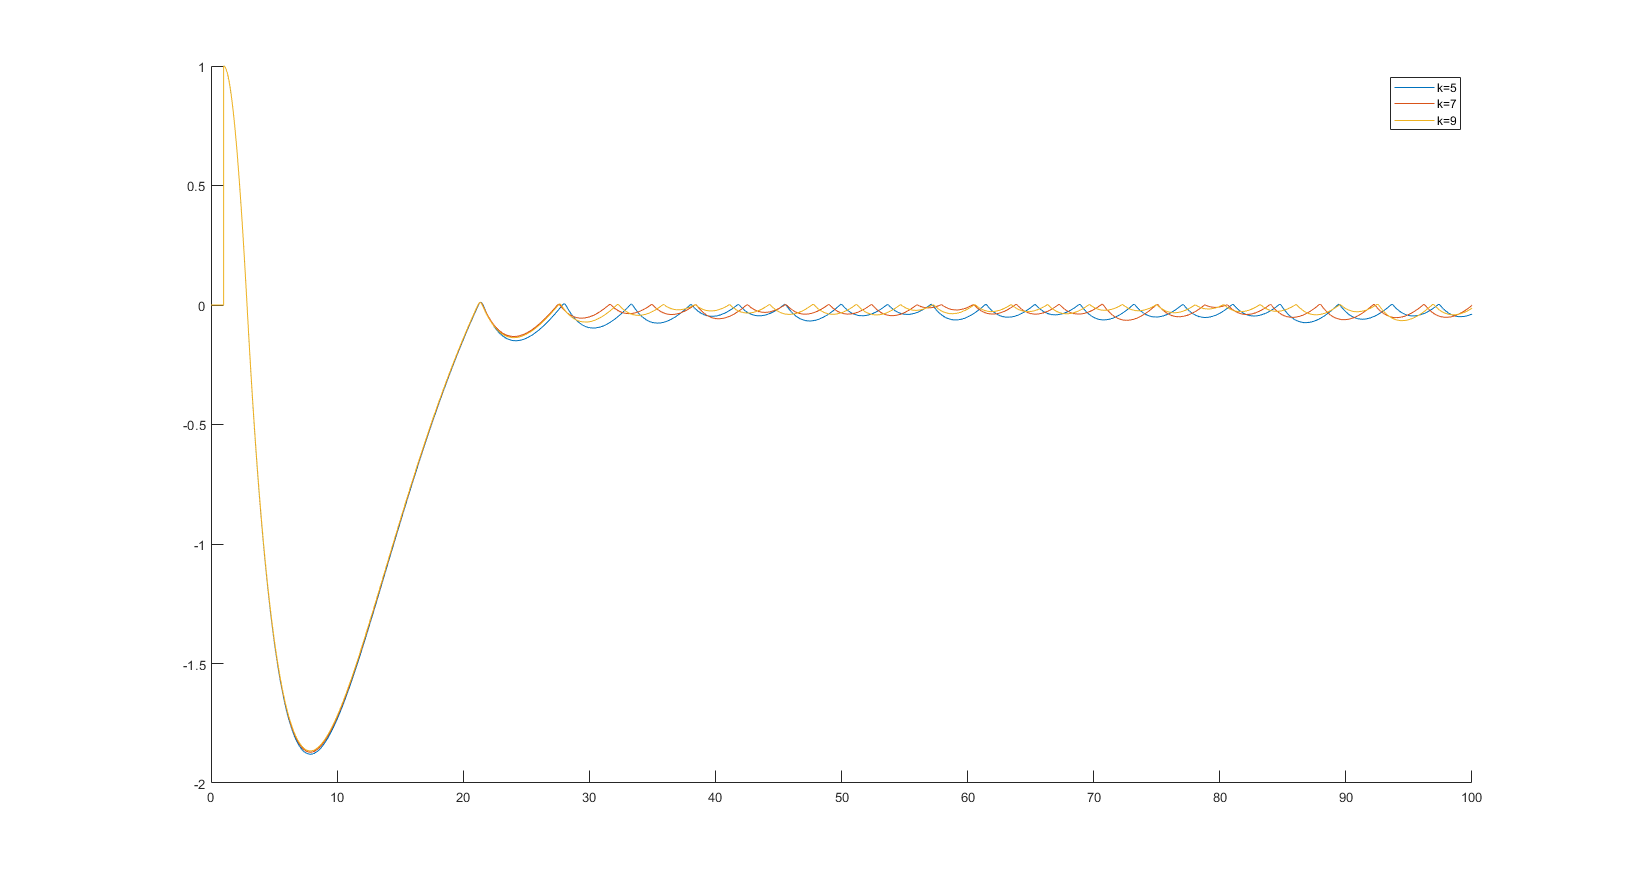
\includegraphics[width=120mm]{dwu_kor_k_bez.png}
	\caption{Zmiana K}
    \label{fig:Rysunek}
\end{figure}


\newpage


		\item Regulator trójpołożeniowy
Do testowania regulatora trójpołożeniowego wykorzystałem poniższe funkcje.

\begin{lstlisting}[caption=Funkcja testująca regulator trójpołożeniowy bez histerezy.]
function testTrojpolozeniowyBezHisterezyKor(start, step, stop)
load_system('trojpolozeniowy_kor.slx');
hold on;
i = 1;

s1 = start;
while(s1 <= stop)
set_param('trojpolozeniowy_kor/Relay1', 'OnSwitchValue', num2str(0));
set_param('trojpolozeniowy_kor/Relay1', 'OffSwitchValue', num2str(0));
set_param('trojpolozeniowy_kor/Relay2', 'OnSwitchValue', num2str(0));
set_param('trojpolozeniowy_kor/Relay2', 'OffSwitchValue', num2str(0));

%set_param('trojpolozeniowy_kor/Transfer Fcn3', 'Denominator', strcat('[',num2str(s1), ' 1]'));
set_param('trojpolozeniowy_kor/Transfer Fcn3', 'Denominator', strcat("[0.1 ", num2str(s1), ']'));


sim('trojpolozeniowy_kor.slx');
figure(1);
%plot(relay.time, relay.signals.values);
plot(e.time, e.signals.values, 'DisplayName', strcat('Tk=', num2str(s1)));
%plot(fun.time, fun.signals.values);
s1 = s1 + step;
i = i +1;
end
hold all;
end
\end{lstlisting}
		
\begin{lstlisting}[caption=Funkcja testująca regulator trójpołożeniowy z histerezą.]
function testTrojpolozeniowyBezHisterezyKor(start, step, stop)
load_system('trojpolozeniowy_kor.slx');
hold on;
i = 1;

s1 = start;
while(s1 <= stop)
set_param('trojpolozeniowy_kor/Relay1', 'OnSwitchValue', num2str(0.8));
set_param('trojpolozeniowy_kor/Relay1', 'OffSwitchValue', num2str(-0.6));
set_param('trojpolozeniowy_kor/Relay2', 'OnSwitchValue', num2str(0.6));
set_param('trojpolozeniowy_kor/Relay2', 'OffSwitchValue', num2str(-0.8));

%set_param('trojpolozeniowy_kor/Transfer Fcn3', 'Denominator', strcat('[',num2str(s1), ' 1]'));
set_param('trojpolozeniowy_kor/Transfer Fcn3', 'Denominator', strcat("[0.1 ", num2str(s1), ']'));


sim('trojpolozeniowy_kor.slx');
figure(1);
%plot(relay.time, relay.signals.values);
plot(e.time, e.signals.values, 'DisplayName', strcat('k=', num2str(s1)));
%plot(fun.time, fun.signals.values);
s1 = s1 + step;
i = i +1;
end
hold all;
end
\end{lstlisting}

\newpage
		
\begin{figure}[!h]
    \centering
	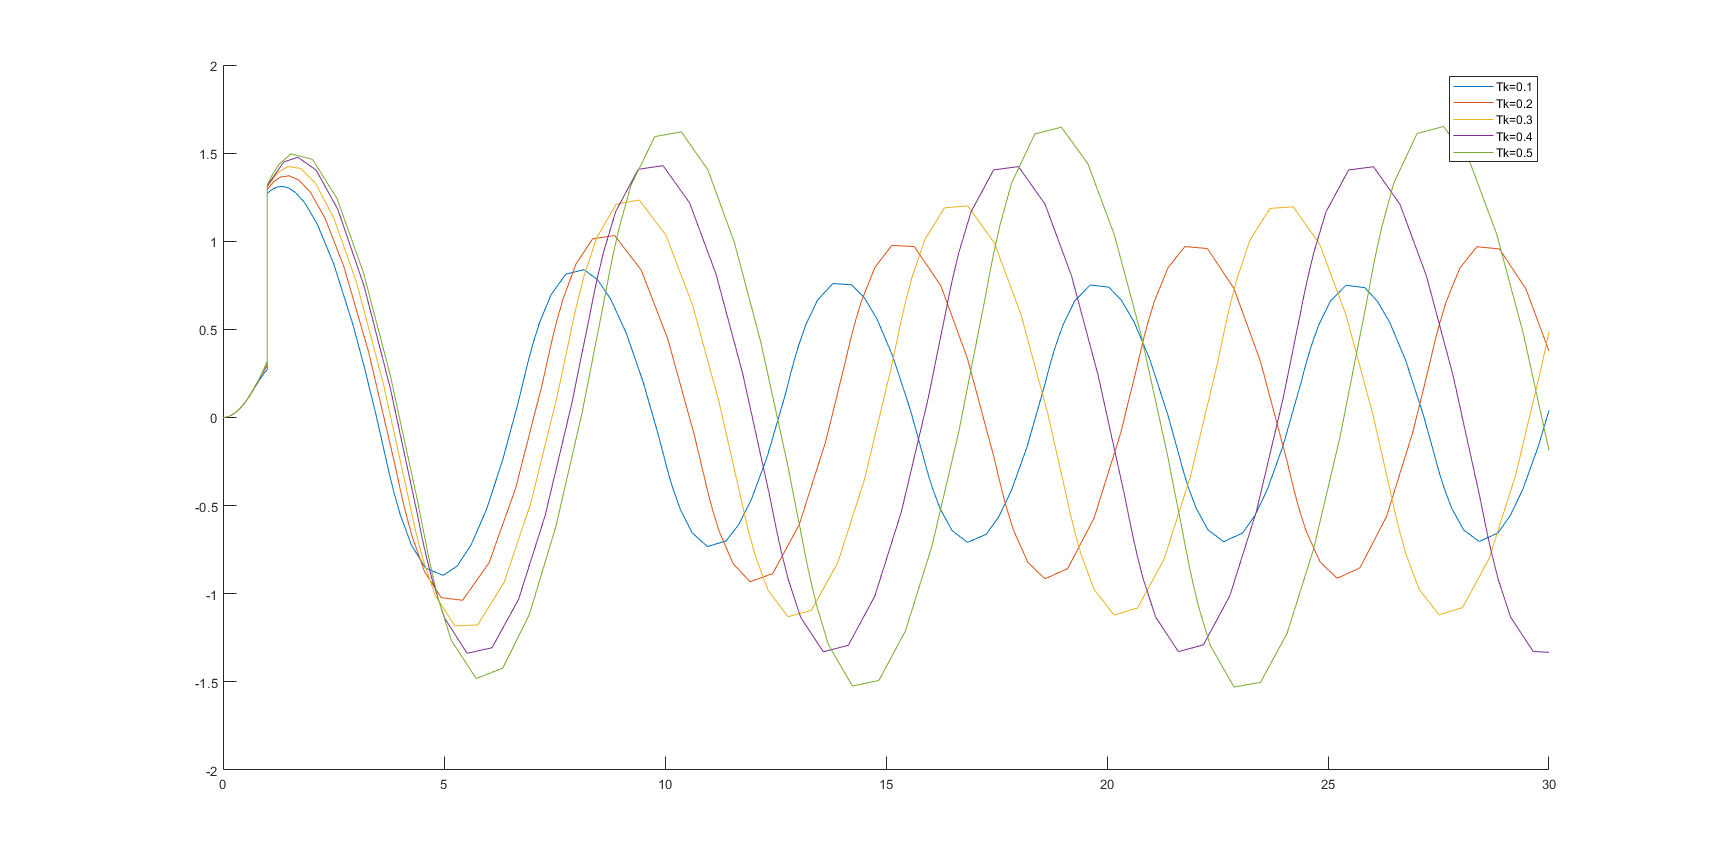
\includegraphics[width=120mm]{troj_kor_tk.png}
	\caption{Regulator trójpołożeniowy z histerezą przy zmianie Tk}
    \label{fig:Rysunek}
\end{figure}

\begin{figure}[!h]
    \centering
	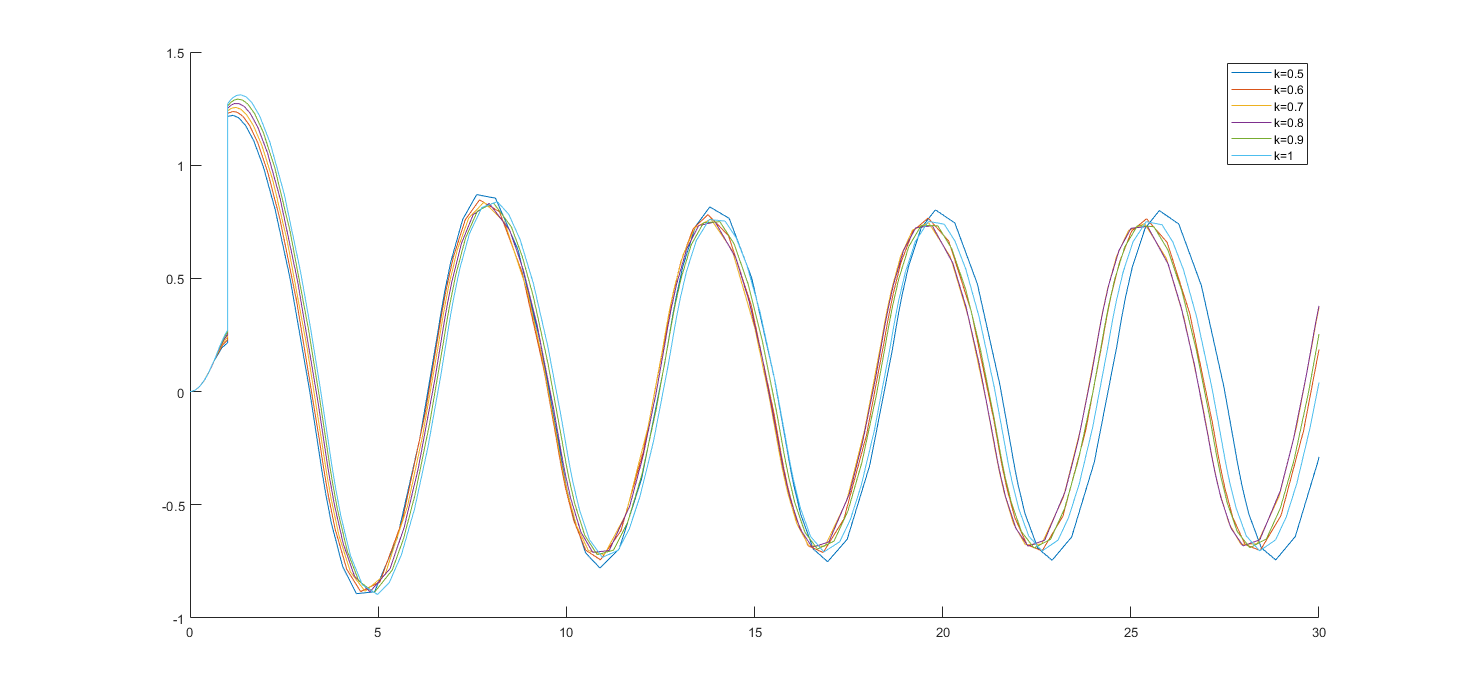
\includegraphics[width=120mm]{troj_kor_k.png}
	\caption{Regulator trójpołożeniowy z histerezą przy zmianie k}
    \label{fig:Rysunek}
\end{figure}

Wybrane parametry to:
Tk=0.1
k=1

\newpage
\newpage
Dla układu bez histerezy wykonałem takie same pomiary.
\begin{figure}[!h]
    \centering
	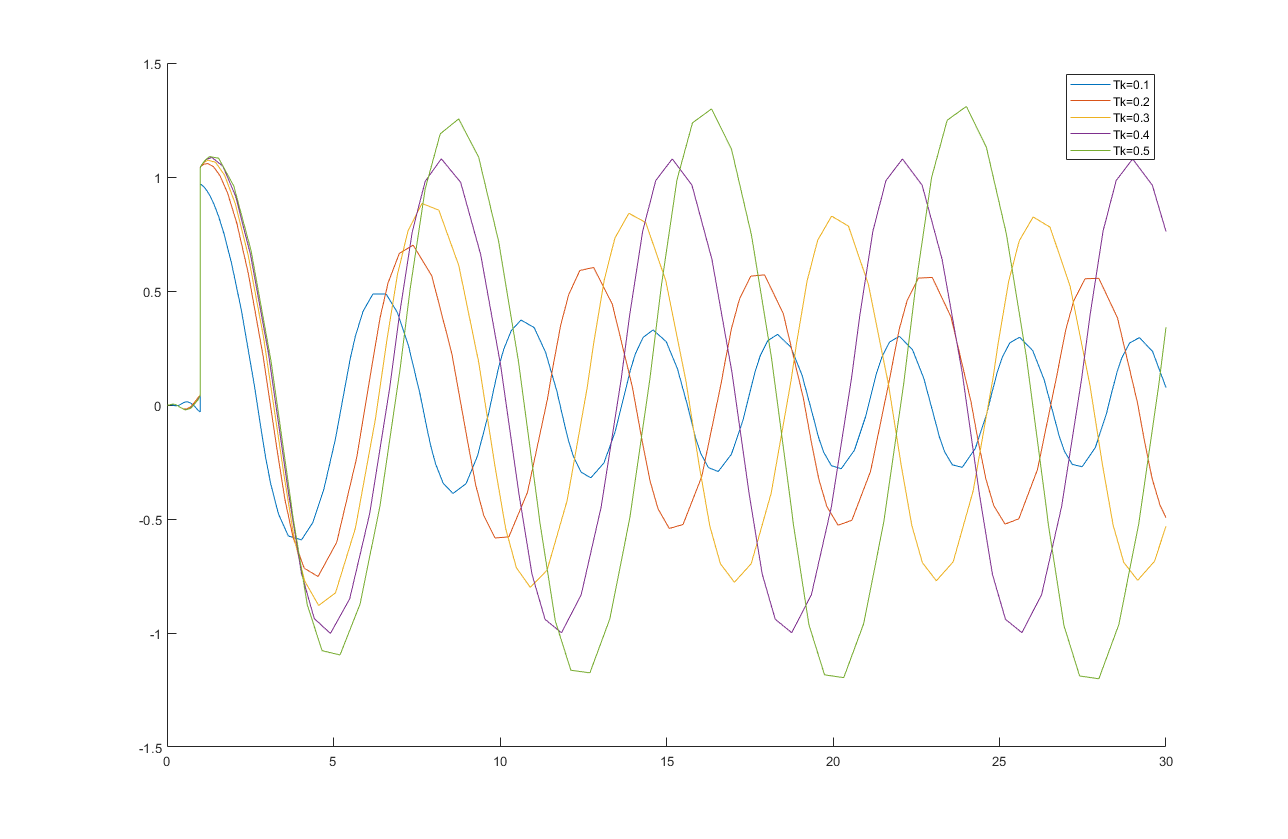
\includegraphics[width=120mm]{troj_kor_tk_bez.png}
	\caption{Regulator trójpołożeniowy bez histerezy przy zmianie Tk}
    \label{fig:Rysunek}
\end{figure}

\begin{figure}[!h]
    \centering
	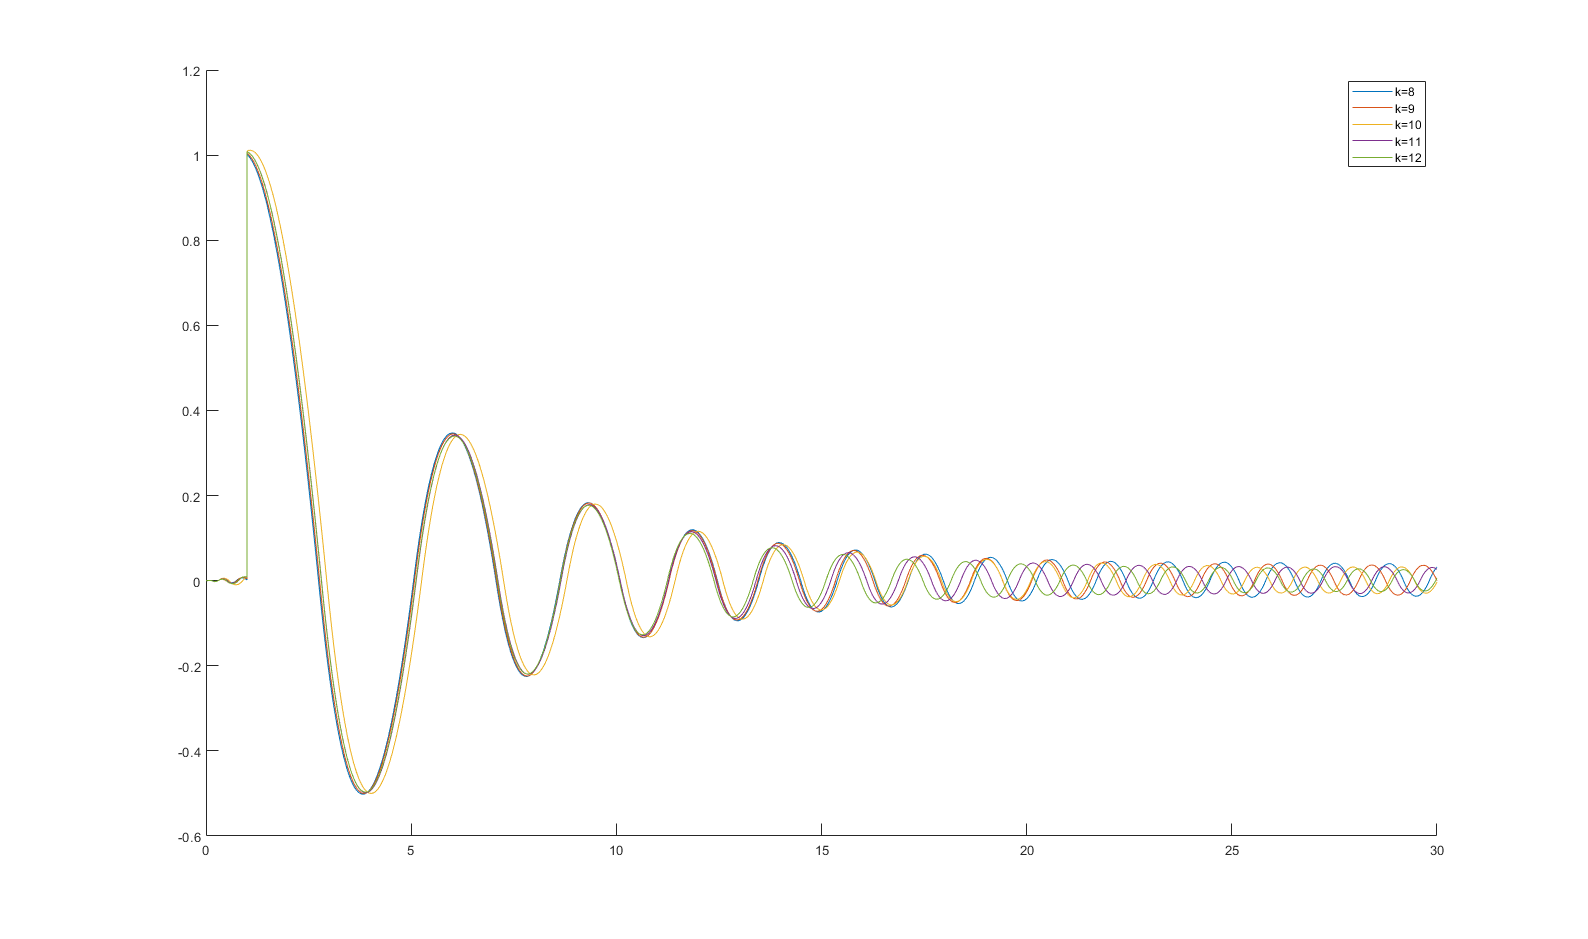
\includegraphics[width=120mm]{troj_kor_k_bez.png}
	\caption{Regulator trójpołożeniowy bez histerezy przy zmianie k}
    \label{fig:Rysunek}
\end{figure}

\end{enumerate}
\newpage
\newpage
\section{Wnioski.}\label{sec:wnioski}
Histereza umożliwia zmieniszenie zużycia sprzętu przez zmniejszenie częstotliwości przełączeń między stanami, kosztem odchyłów od pożądanych wartości. Wybór zakresu histerezy zależy od systemu w którym działa regulator oraz od tego jakiej dokładności wyjściowej wymaga.

Regulator trójpołożeniowy pozwa na określenie 3 stanów, dzięki którym uzyskujemy większą kontrolę nad działaniem systemu.

Człon korekcyjny pozwala dostosować system do naszych potrzeb, wpływa on na zmianę częstotliwości przęłączania.

\end{document}